\chapter{Experiment 3: Relearning a task}
\label{exp3}

\begin{figure}[hb]
    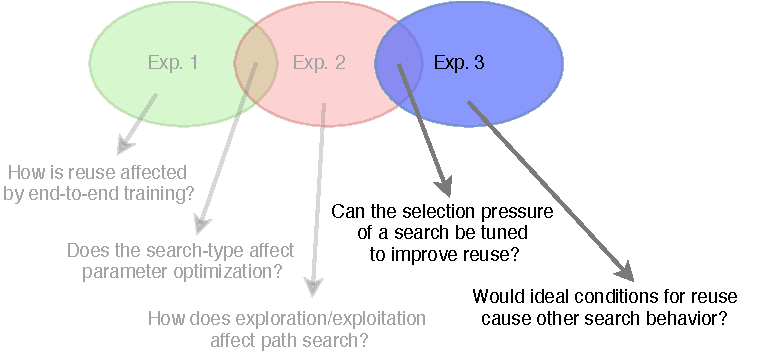
\includegraphics[width=\textwidth]{Chapters/4.Experiments/exp3/figures/exp3.pdf}
    \caption[Experiment focus]{Visualization of how the questions in this chapter fit in the larger context of this thesis.}
    \label{fig:exp3.questions}
\end{figure}
\noindent
The motivation behind reusing modules is, as mentioned in the introduction, to increase the number of tasks a PathNet can learn by decreasing the amount of new capacity a path needs to allocate for a new task. An optimal search algorithm for new paths should therefore be able to reuse as much knowledge as possible without limiting the performance. If we assume an ideal search algorithm would find optimal modules for each task, it should be able to find and reuse all learned knowledge if a task is learned twice. 

This is put to the test by learning some task twice for all seven algorithms in chapter \ref{exp2}. As the amount of module reuse in these experiments was small, the proverbial "bar" is lowered by reducing the module search space.

The experiments in this chapter relates to those in chapter \ref{exp1} and \ref{exp2} as seen in figure \ref{fig:exp3.questions}, and will attempt to answer:
\begin{itemize}
    \item \emph{"Given optimal conditions for module reuse, which selection pressure scheme is best suited for reusing knowledge?"}
\end{itemize}


\section{Description}
The experimental structure here is the same as in chapter \ref{exp2} with two differences. The maximum tournament size used is 10 instead of 25, and the tasks trained on is two cases of a full cSVHN classification problem with all ten classes. This is to create optimal\footnote{Optimal conditions here means learning a task where a full set of parameters is already optimized for that task.} conditions for module reuse. After searching for an optimal path for both tasks, the module reuse for the second task is noted. 

By performing this experimental trial for each algorithm multiple times, we can compare the observations of reuse with the probability of seeing these results when randomly selecting modules, and then with each other. 

\section{Hypothesis}
Based on the reuse in the previous selection pressure experiments, we do not expect any algorithm to yield perfect results\footnote{Perfect results here would constitute finding all modules used in the previous path.}, but instead have a statistically significant difference from random module selection. Given the algorithms different selection pressures, they are expected to give somewhat different reuse results.

As each search should be capable of reaching a decent validation accuracy on its own, it is not expected that there will be a significant difference between task 1 and task 2 for any of the algorithms. However, there is no reason to believe the effects the different tournament sizes have on accuracy will be any different than in chapter \ref{exp2}. 

\section{Experimental setup}
\label{exp3:implementation}
The experiment structure here is a binary task problem, where we want to find two paths for a full cSVHN classification problem twice, meaning both task 1 and task 2 is cSVHN classification with all classes. The two searches should have a non-zero probability of zero reuse, so the PathNet dimensions are set to 3 layers of 6 modules each with a maximum of 3 active modules per layer. We can describe the total number of possible paths as 
\begin{equation*}
    \prod_{i=0}^{\omega-1}(M-i)^{L}
\end{equation*}
where \(\omega\) is the maximum number of active modules in each layer for each path, \(M\) is the number of modules in each PathNet layer, and  \(L\) is the number of layers in the PathNet. This means the number of possible paths in a 20-by-3 PathNet with \(\omega=3\) is  
\begin{equation*}
    \prod_{i=0}^{3-1}(20-i)^{3}\approx 3.2\times10^{11}
\end{equation*}
and in this experiment
\begin{equation*}
    \prod_{i=0}^{3-1}(6-i)^{3}\approx 1.7\times10^{6}
\end{equation*}
Reducing the PathNet size from 20 to 6 modules in each layer have reduced the search space with five orders of magnitude, and it should, therefore, be significantly easier to find reusable modules here than in the previous experiment.

\begin{table}[ht]
    \centering
    \begin{tabular}{clll}
    \# of reuse & \# of outcomes & Monte-Carlo probabilities & Rounded  \\
    0           & 88892859      & 0,088892859               & 0,0888928 \(\pm 10^{-7}\)  \\
    1           & 266671854     & 0,266671854               & 0,2666718 \(\pm 10^{-7}\)  \\
    2           & 327560805     & 0,327560805               & 0,3275608                  \\
    3           & 213925123     & 0,213925123               & 0,2139251                  \\
    4           & 81393230      & 0,08139323                & 0,0813932                  \\
    5           & 18720470      & 0,01872047                & 0,0187205                  \\
    6           & 2612531       & 0,002612531               & 0,0026125                  \\
    7           & 213747        & 0,000213747               & 0,0002137 \(\pm 10^{-7}\)  \\
    8           & 9195          & 0,000009195               & 0,0000092                  \\
    9           & 186           & 0,000000186               & 0,0000002                 
    \end{tabular}
    \caption{Results from Monte-Carlo approximation of reuse probabilities for two paths in a 6-by-3 PathNet with a maximum of 3 active modules in each layer.}
    \label{tab:montecarlo}
\end{table}

We can approximate the probability of finding any number of reuse by randomly selecting two paths within the limitations of the PathNet dimensions and path-size with a Monte-Carlo approach. Using equation \ref{eq:montecarloP} where we want the probabilities to be minimum ten times as large as the standard deviation (\(R=0.1\)) and \(n=10^{9}\) Monte-Carlo trials, the probability "accuracy" is calculated to be
\begin{equation*}
    \frac{1}{nR^{2}+1}=\frac{1}{10^{7}+1}\approx10^{-7}
\end{equation*}
Meaning we can tell the probability of reuse to the seventh decimal place from the Monte-Carlo results. The results of the performed Monte-Carlo estimation can be found in table \ref{tab:montecarlo}.

The expected reuse distribution is calculated based on the Monte-Carlo estimated probabilities, and Mann-Whitney tests are used to see how the algorithms module reuse holds up compared to expectations.

Learning from the conclusion in chapter \ref{exp2}, the algorithms maximum tournament size is reduced from 25 to 10.

\section{Results}

\subsection{Population Diversity}
\begin{figure}[!ht]
    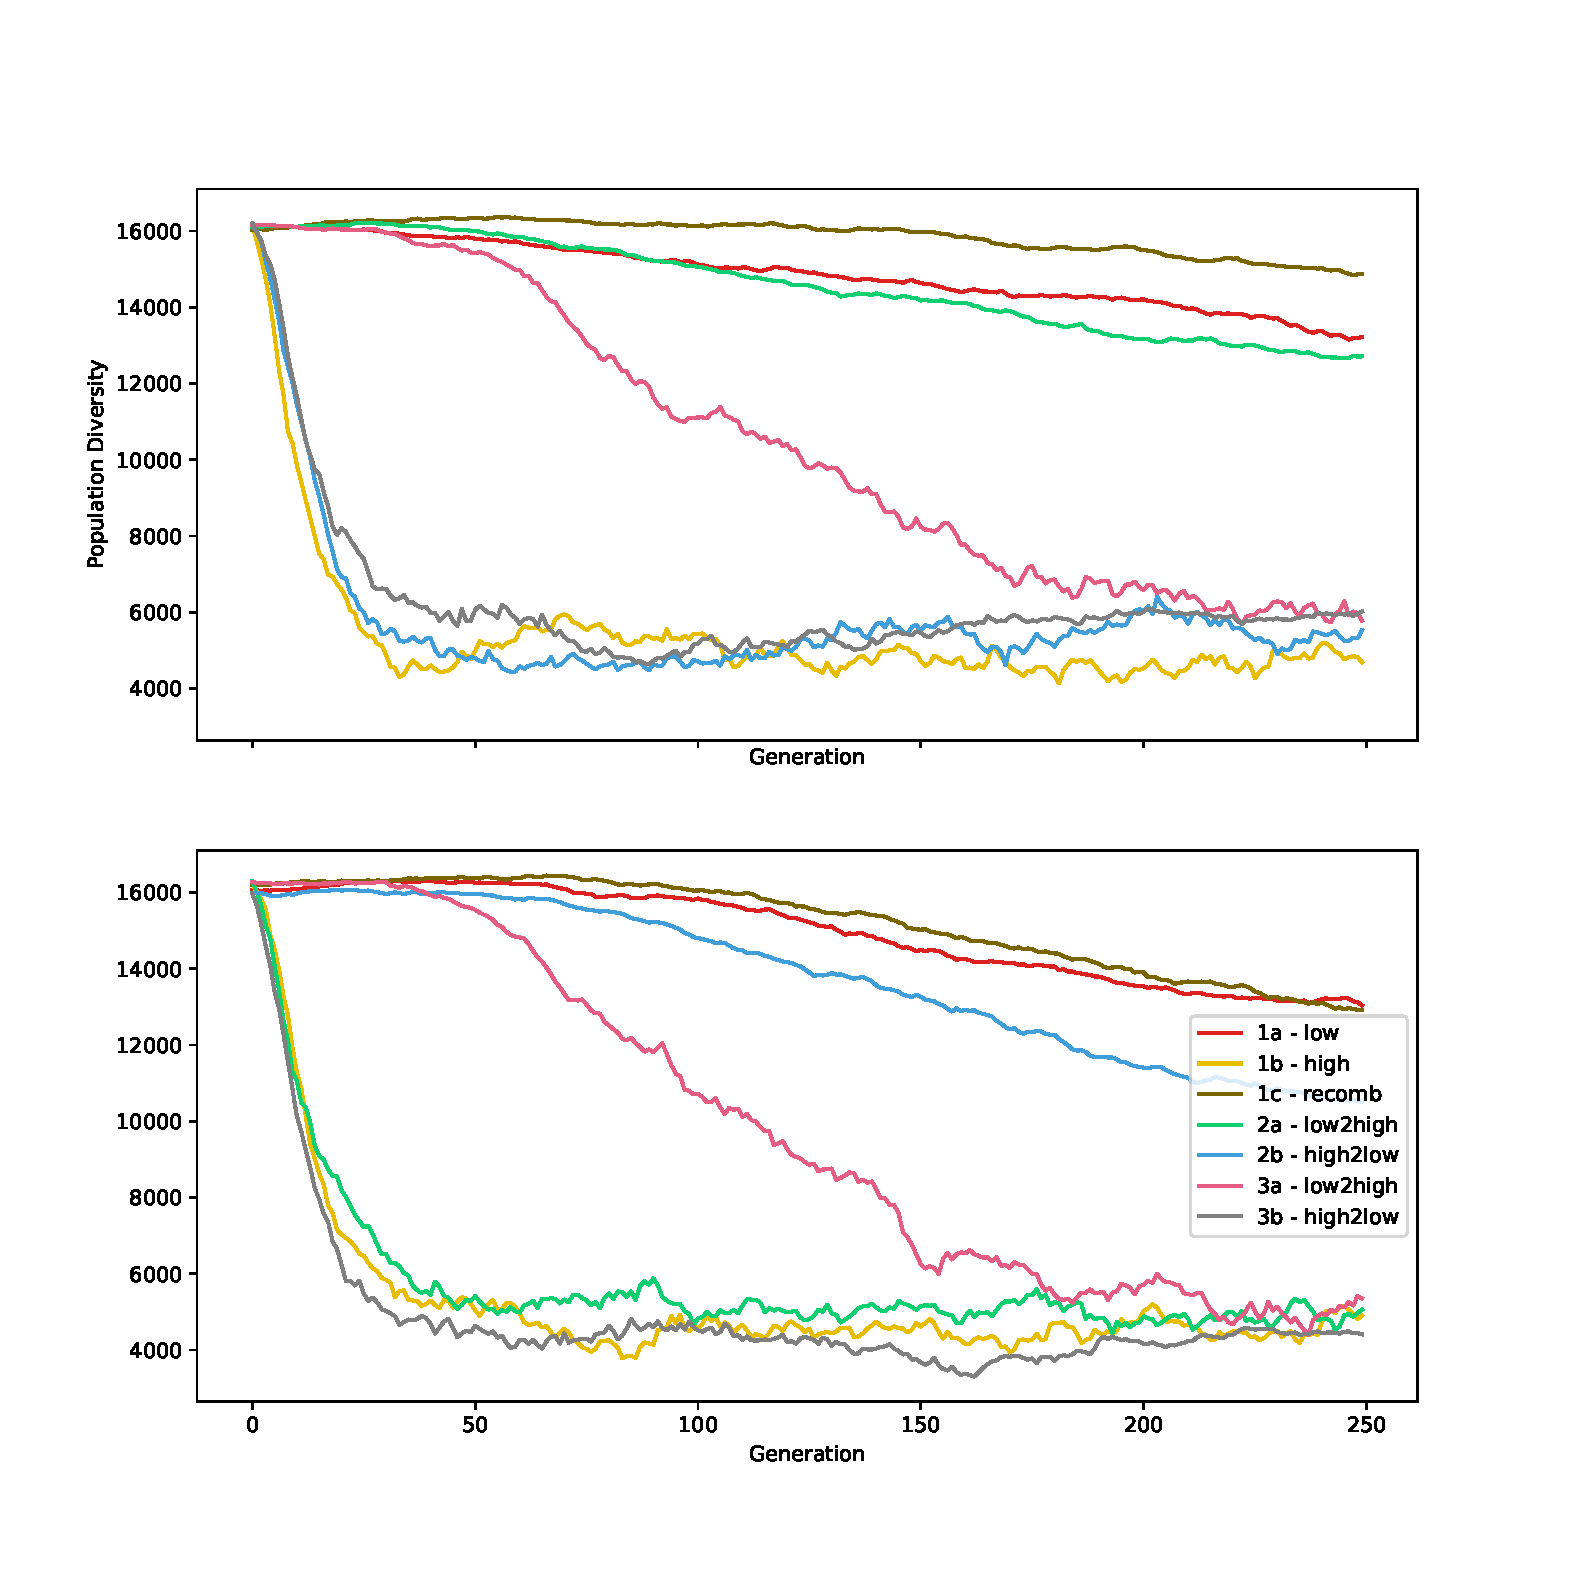
\includegraphics[width=\textwidth, center]{Chapters/4.Experiments/exp3/figures/diversity_hamming.pdf}
    \caption[Hamming diversity plot]{The average pair-wise Hamming distance diversity for each algorithm over 250 generations.}
    \label{fig:exp3.hamming}
\end{figure}
\begin{figure}[!ht]
    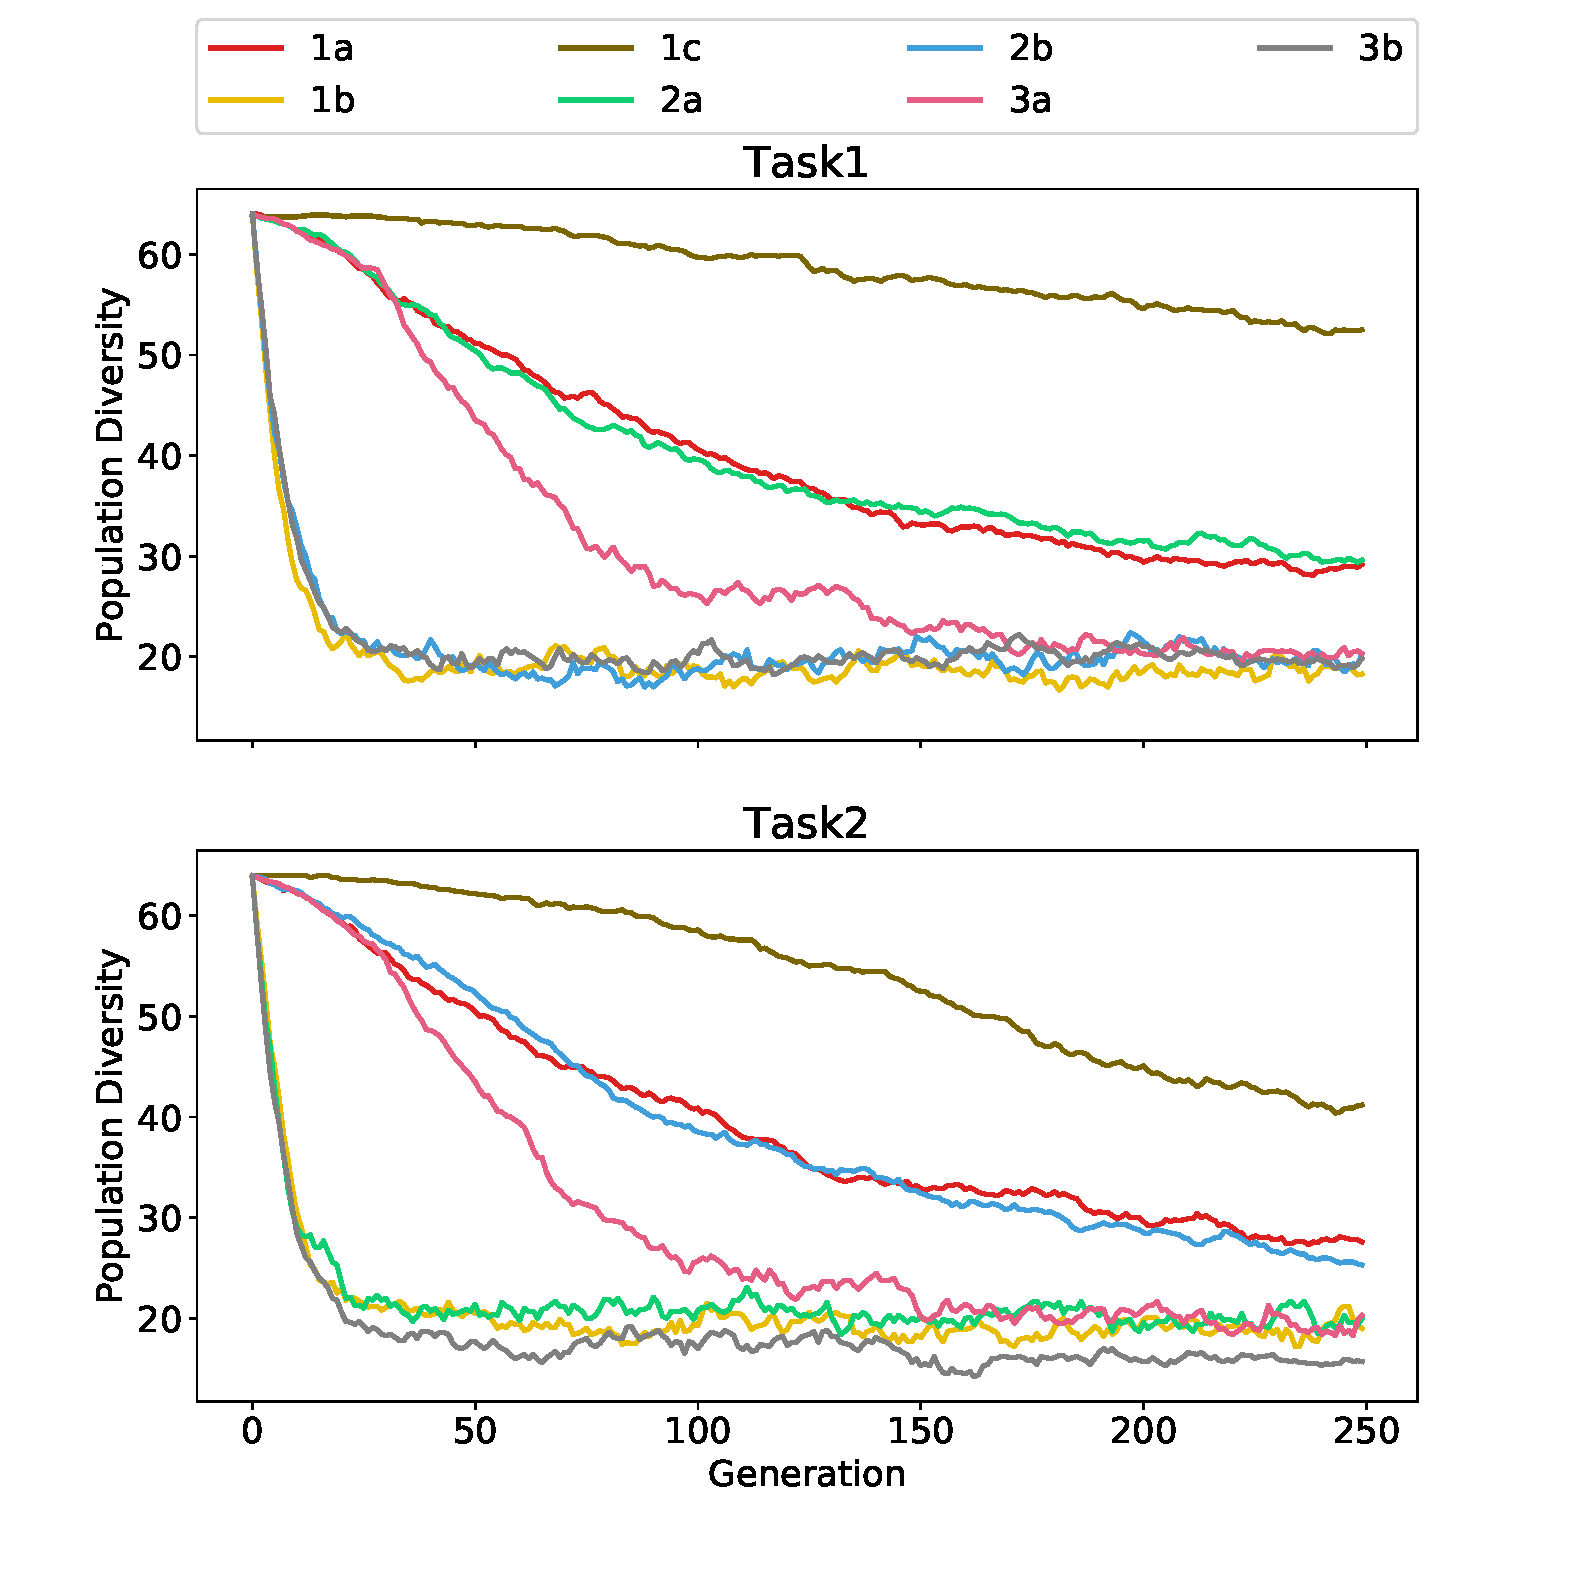
\includegraphics[width=\textwidth, center]{Chapters/4.Experiments/exp3/figures/diversity_frequency.pdf}
    \caption[Frequency diversity plot]{The average amount of unique paths for each algorithm over 250 generations.}
    \label{fig:exp3.frequency}
\end{figure}

As the algorithms that run here are the same as in chapter \ref{exp2}, the convergence rates in figures \ref{fig:exp3.hamming} and \ref{fig:exp3.frequency} are quite similar to what we saw in section \ref{exp2:diversity}. However, the searches are run for 250 generations, which let the diversity of algorithms with low selection pressure converge further.

What is noteworthy about these diversity plots is that algorithm 1c in both cases converge more within the 250 generations for task 2 than task 1. Testing the null-hypothesis that the final generations population have a similar pair-wise Hamming distance for task 1 and task 2 gives a p-value of 0.00229 for a one-sided Mann-Whitney test. Confirming the observation is not due to an outlier in the data, but rather a difference in the diversity distributions. The only other algorithms that change their convergence between task 1 and task 2 are algorithms 2a and 2b for obvious reasons.  

\subsection{Modular reuse}
\begin{sidewaysfigure}[p!]
    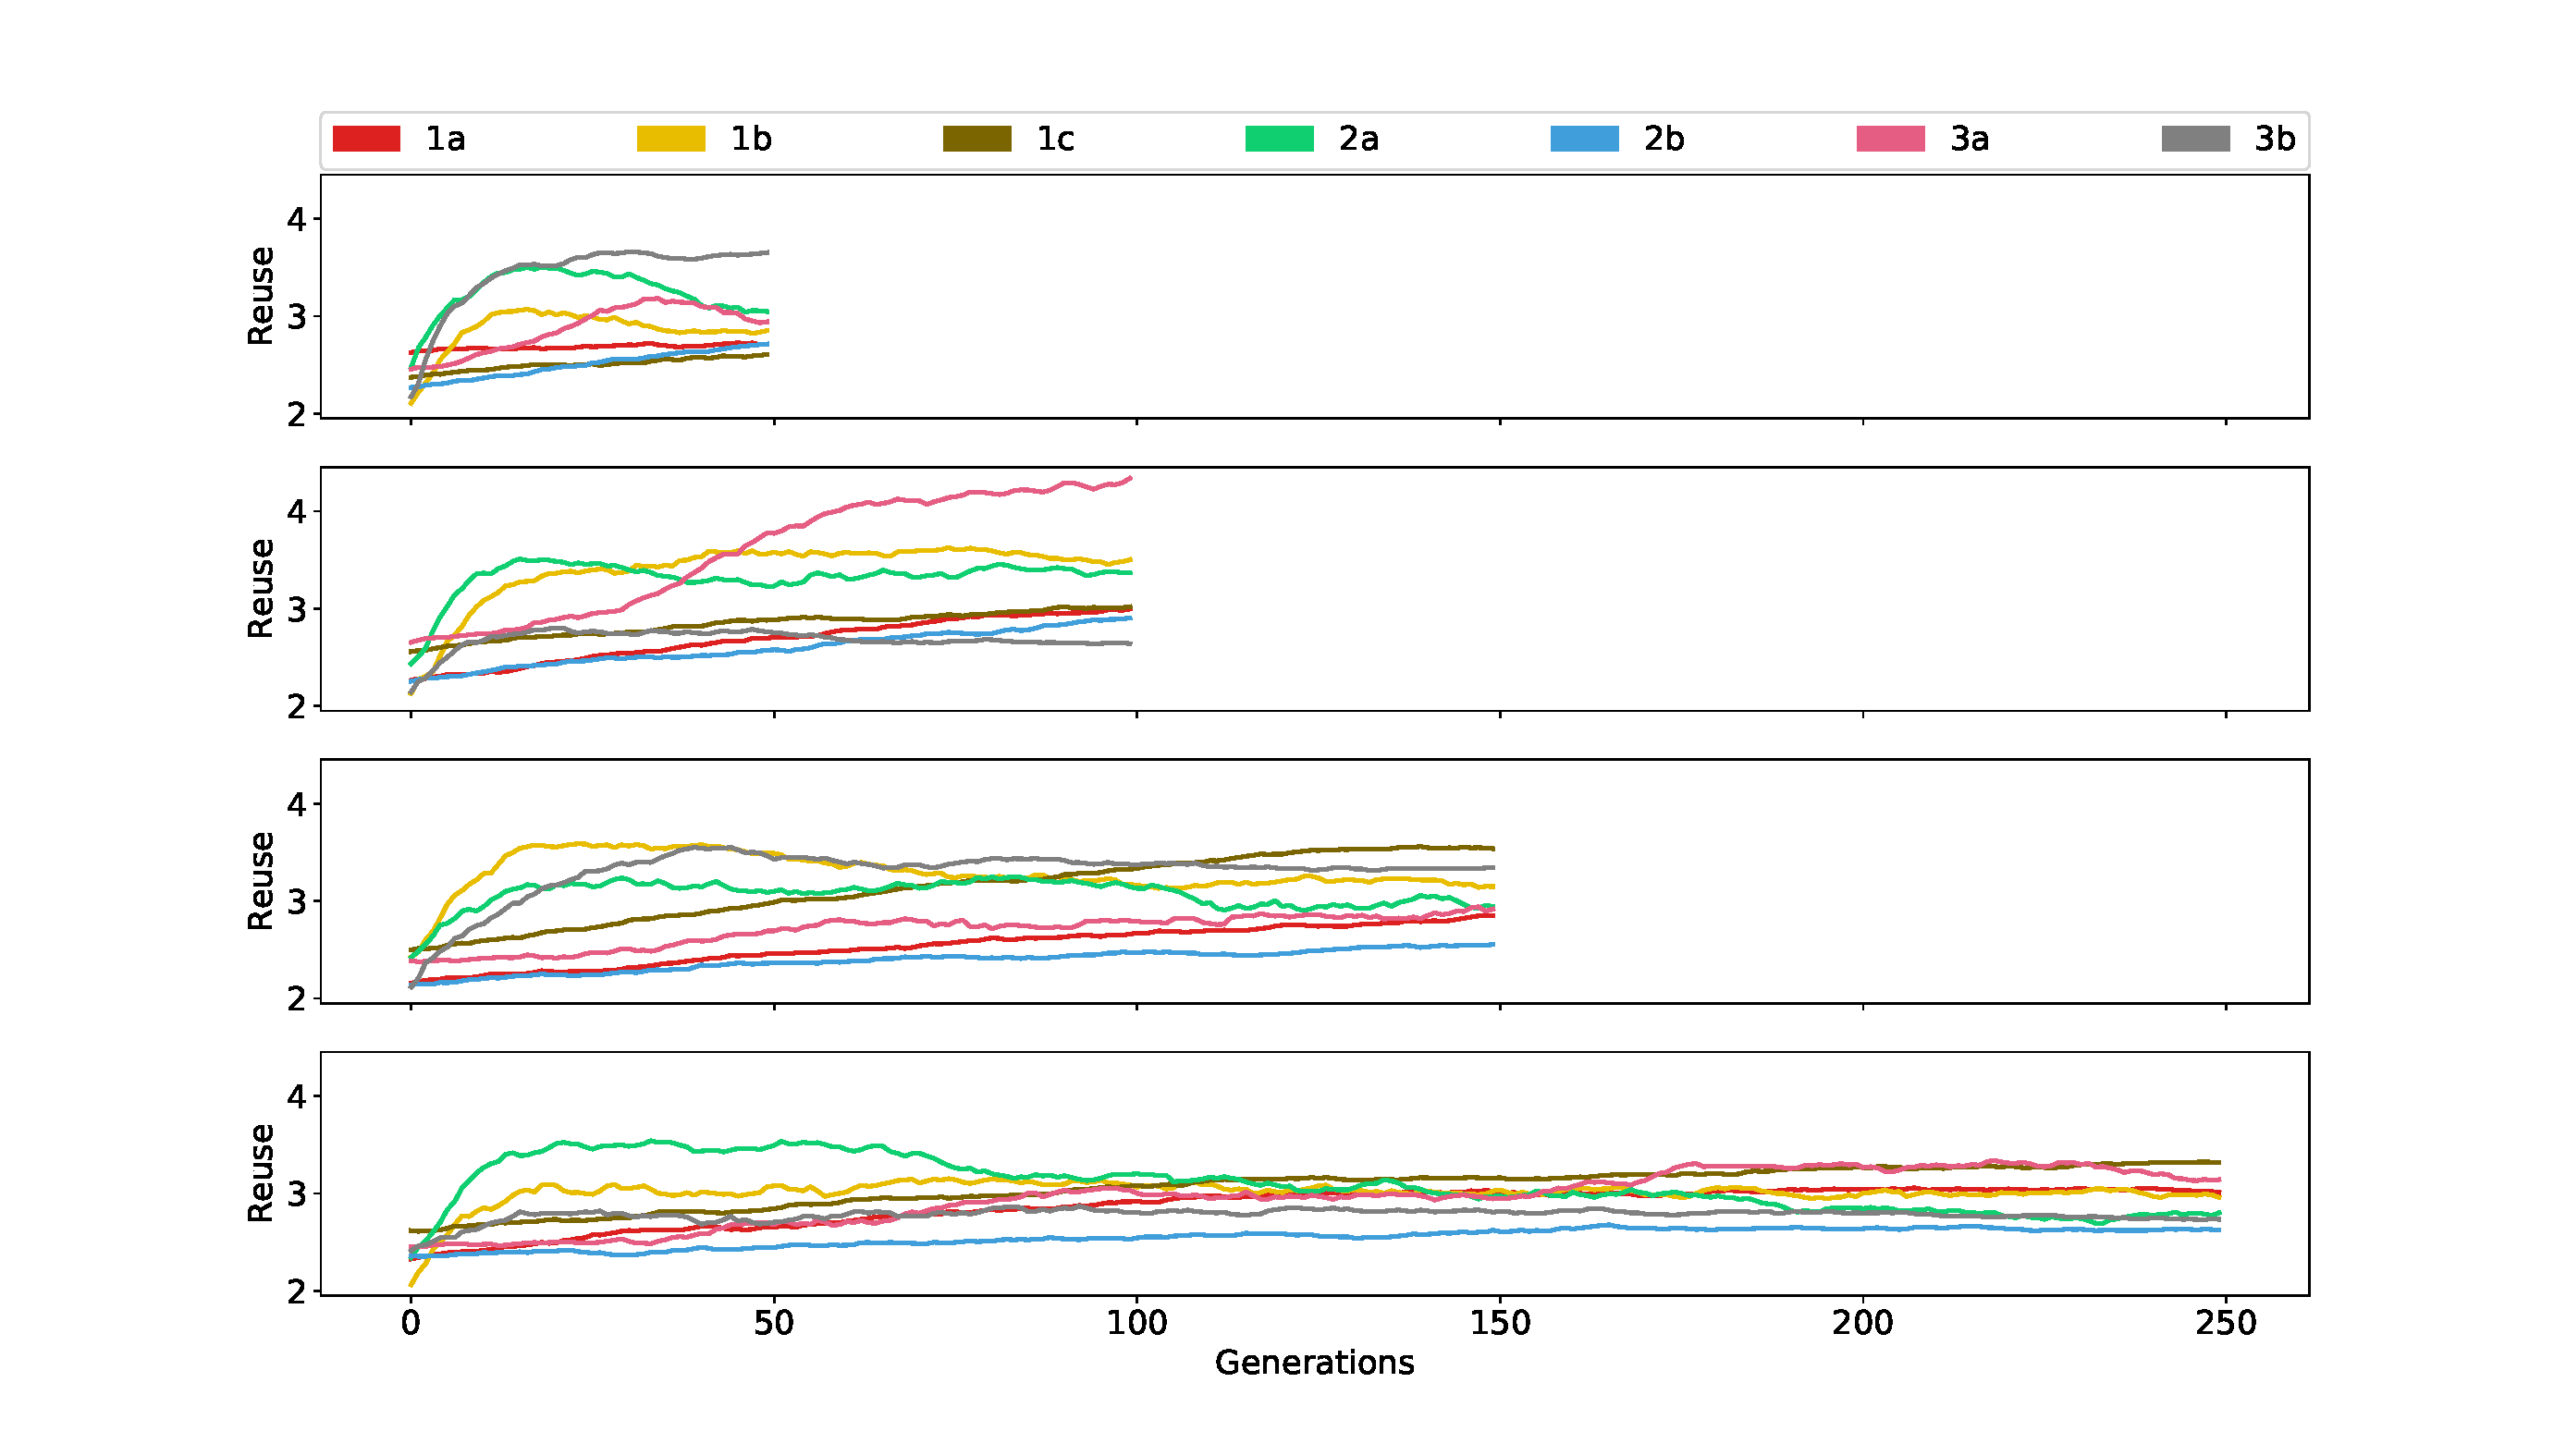
\includegraphics[width=1.2\textwidth, center]{Chapters/4.Experiments/exp3/figures/reuse_progression.pdf}
    \caption[Module reuse during search]{The change in reuse plotted over the search duration. Four generation limits were used, but the reuse during search are expected to be the same across the different search termination limits.}
    \label{fig:exp3.reuseprogression}
\end{sidewaysfigure}
\begin{sidewaysfigure}[ht]
    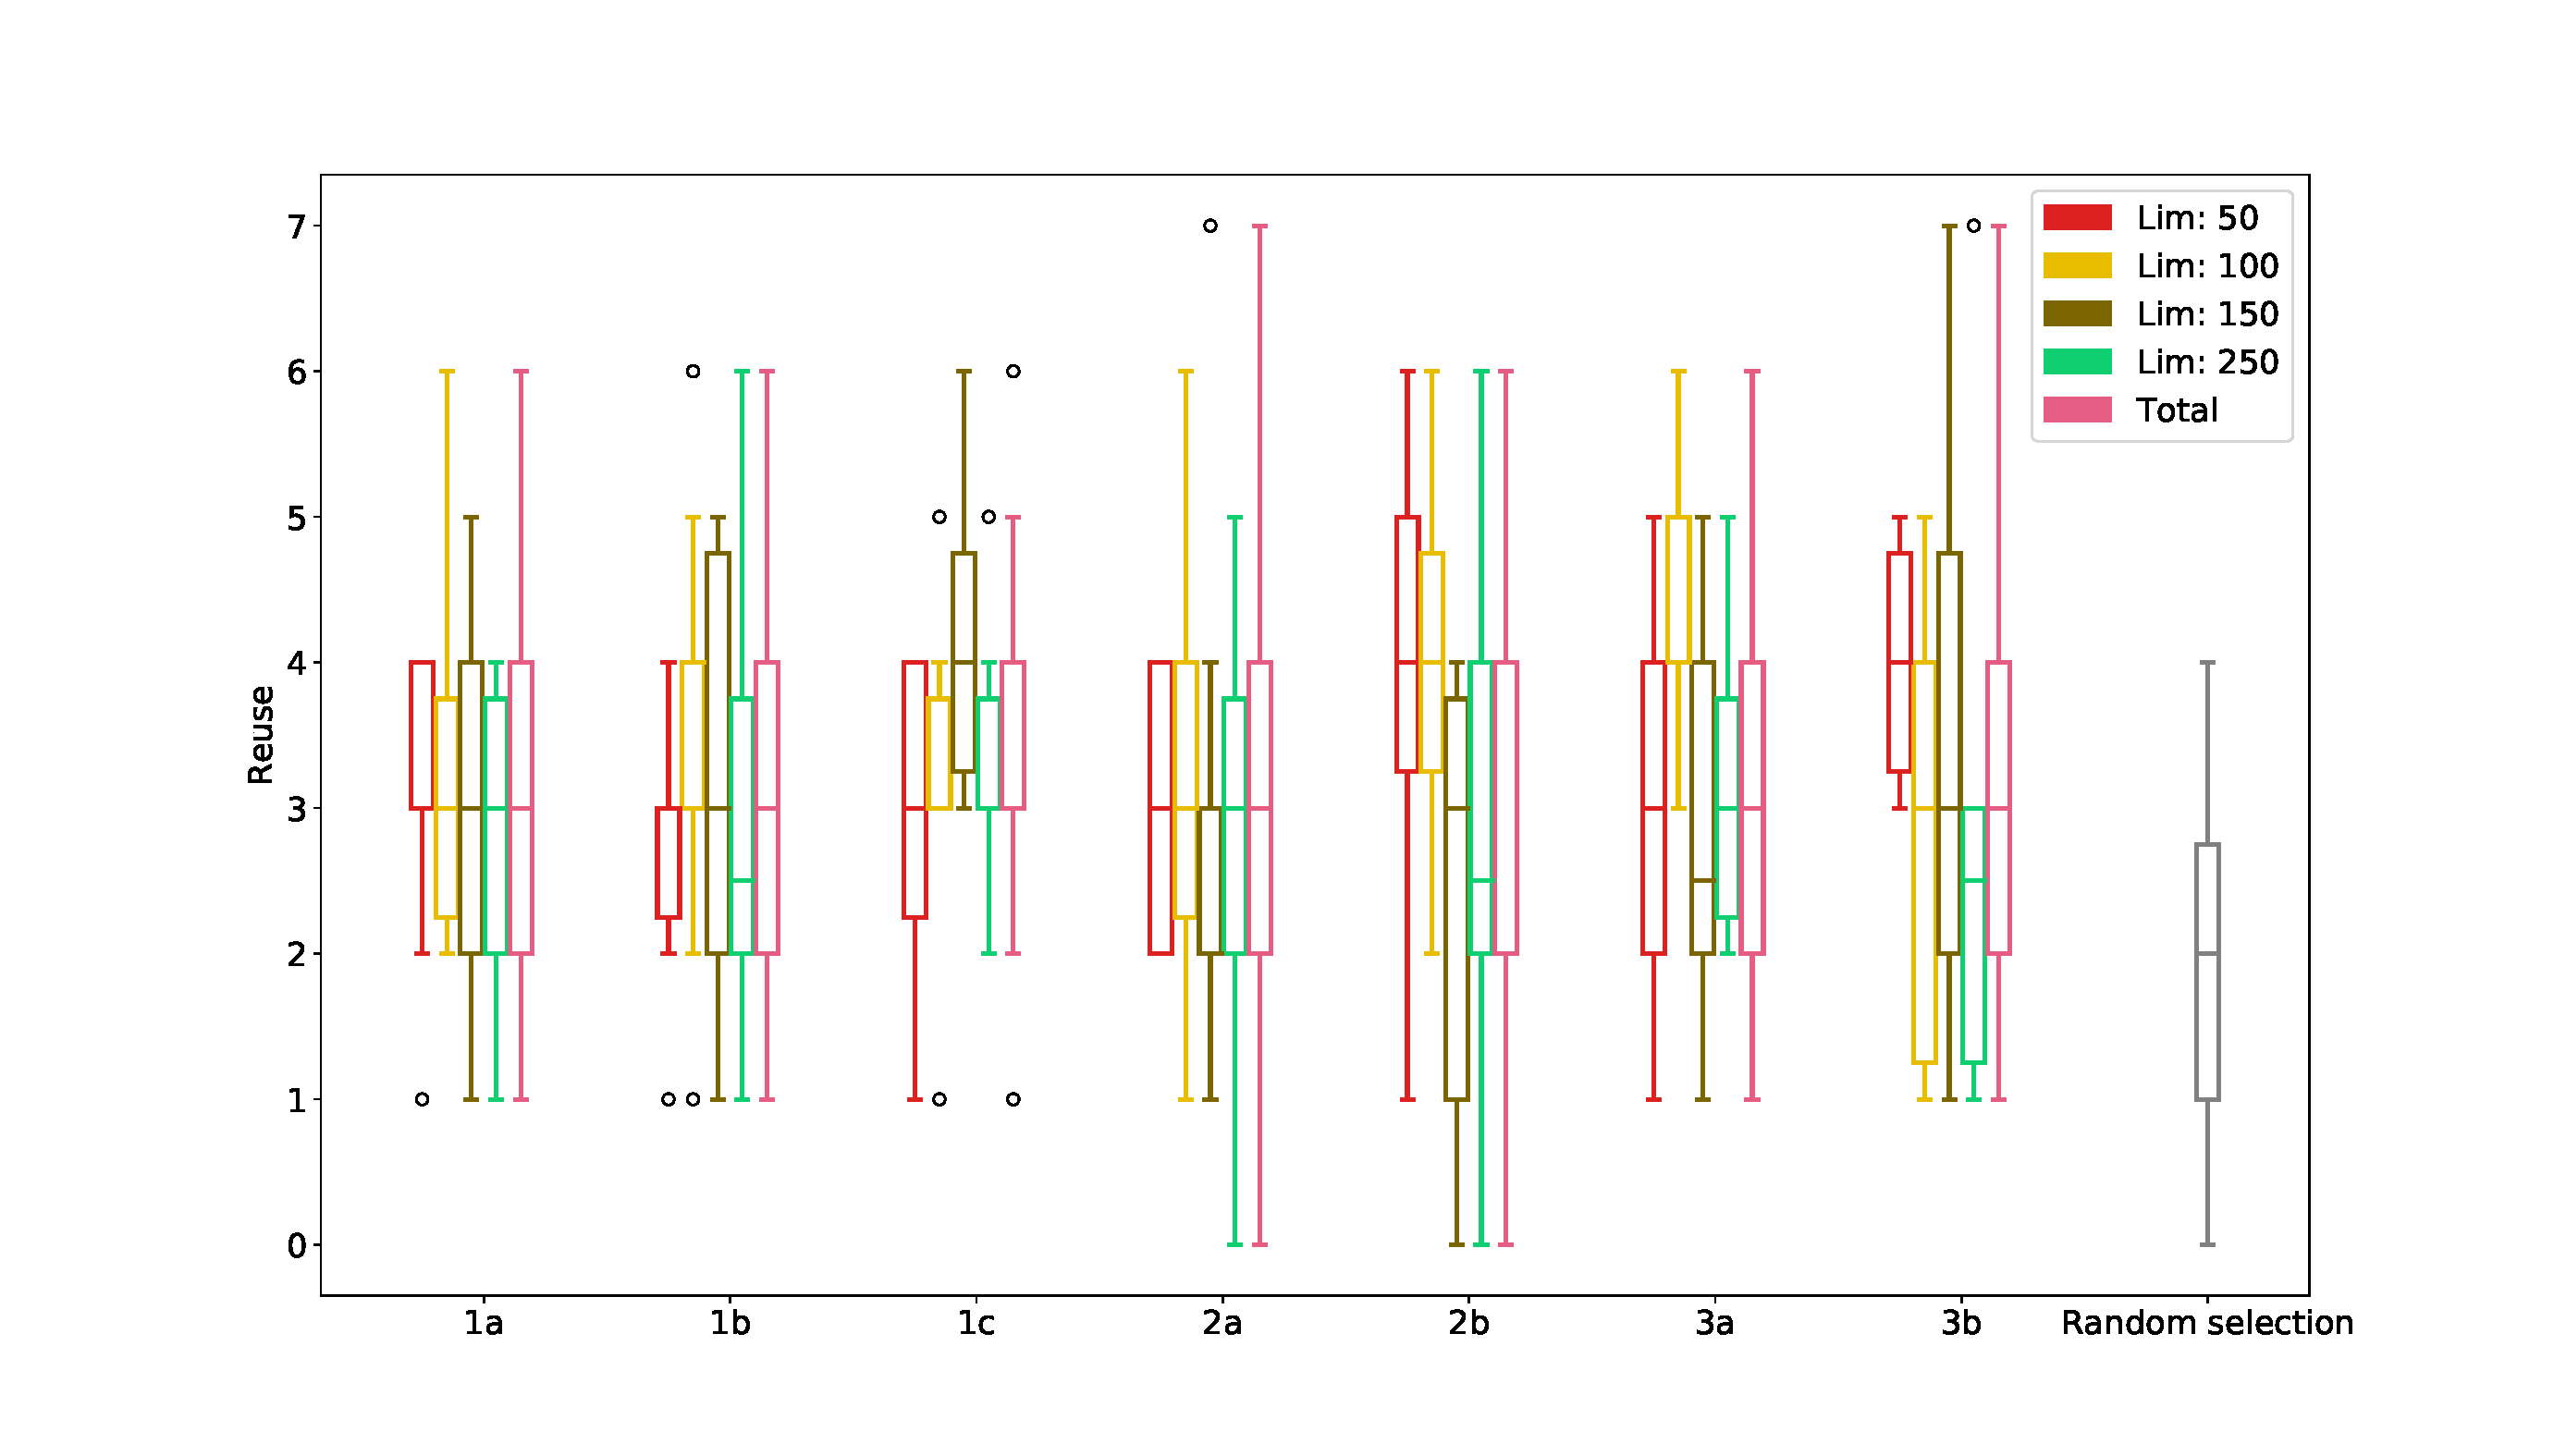
\includegraphics[width=1.25\textwidth, center]{Chapters/4.Experiments/exp3/figures/reuse_boxplot.pdf}
    \caption[Module reuse boxplot]{The module reuse for each algorithm group. The reuse for each generation limit is presented, as well as the reuse for all experimental trials, regardless of search length.}
    \label{fig:exp3.reuseboxplot}
\end{sidewaysfigure}

Figure \ref{fig:exp3.reuseprogression} show the average reuse for each algorithm changing during the searches with different termination limit. Algorithms with high reuse for the second task (1b and 2b) reach the highest level of reuse within the first 30 generations, at which point it starts to drop. Algorithms using a low tournament size instead gradually increase in reuse, where it looks to surpass the other algorithms around 100 generations.  

The box-plot in figure \ref{fig:exp3.reuseboxplot} show the reuse in the optimal paths selected for task 2. The plot does not unveil any major differences in reuse, and an MWW-test of the total reuse distributions for each algorithm show there is no significant differences between the algorithms. However, as the resulting p-values in table \ref{tab:exp3.reuseptable} shows, all algorithms are significantly different from the estimated reuse for random module selection. 

Running the number of MWW-tests needed to compare the individual termination limits for each algorithm with each other would require such a large Bonferroni correction of the \(\alpha\) level that the differences most likely would be found to be not significant. Therefore the statistical analysis of the reuse-results is limited to this comparison of reuse between the groups for all termination limits.

\subsection{Path fitness}
\begin{sidewaysfigure}[ht]
    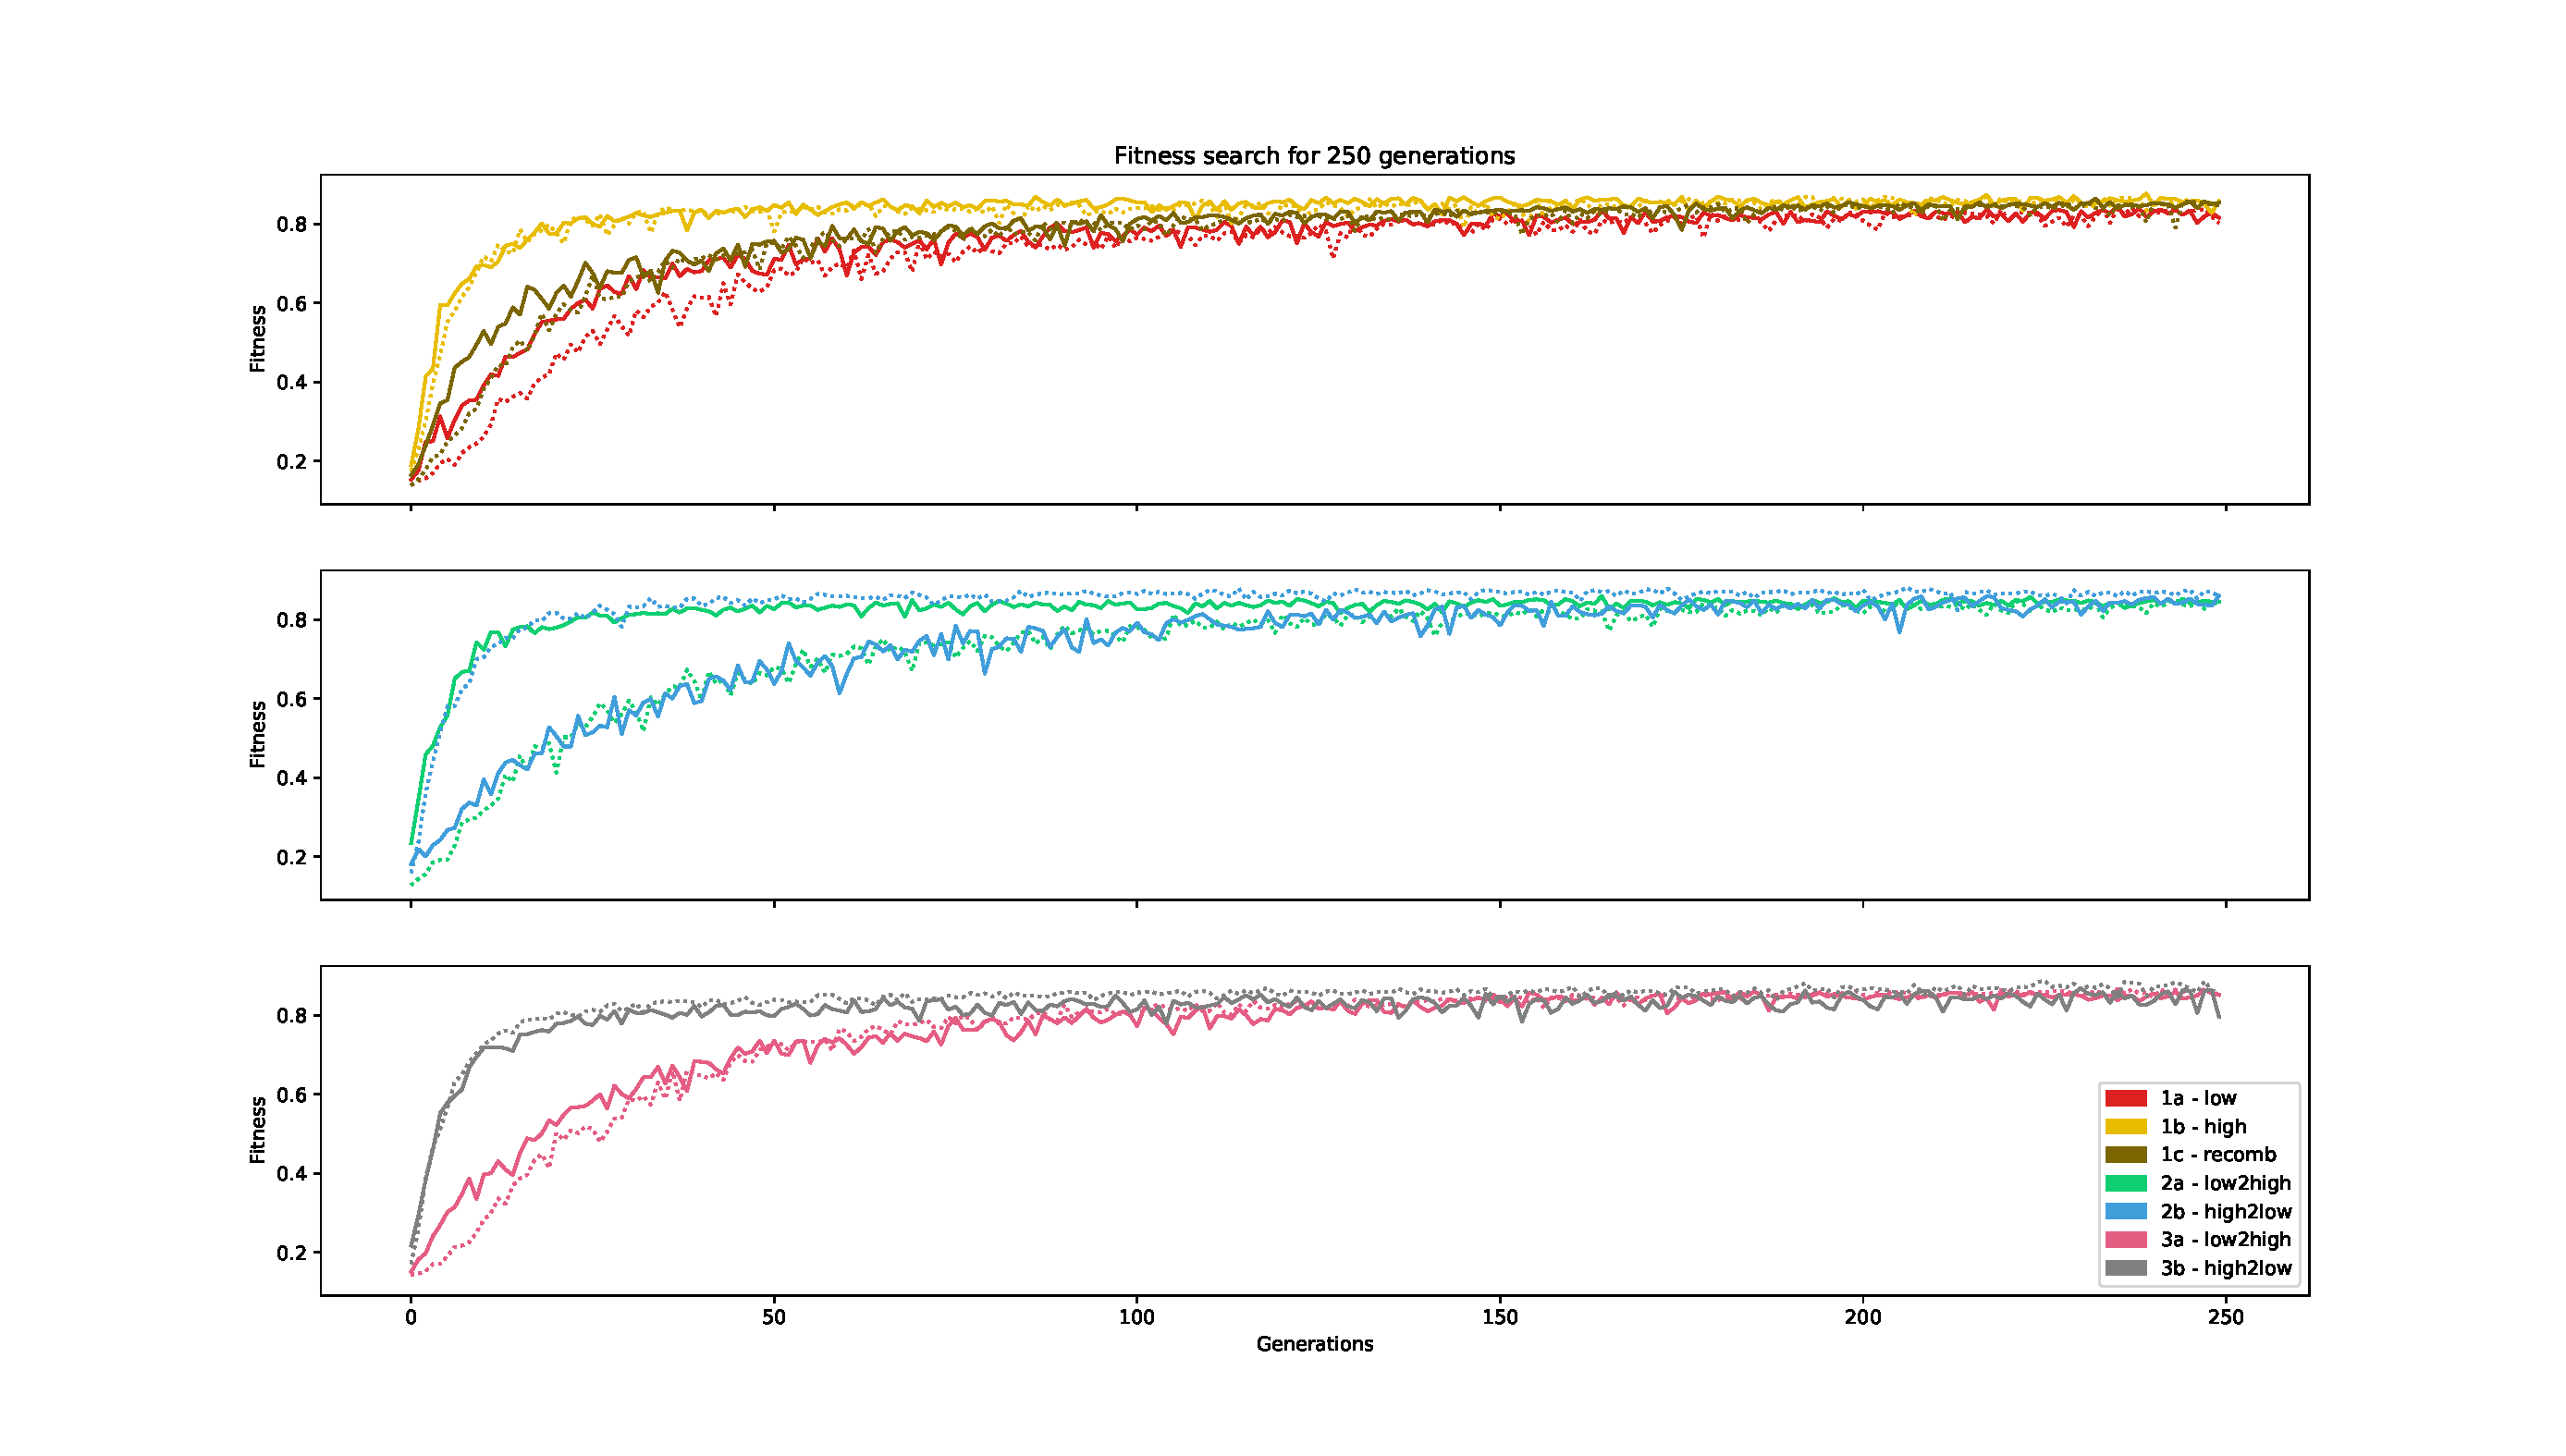
\includegraphics[width=1.25\textwidth, center]{Chapters/4.Experiments/exp3/figures/fitness_progression.pdf}
    \caption[Changes in average tournament fitness]{The average tournament fitness for each generation. The dotted lines are average fitness during search for task 1, while the whole lines are for task 2.}
    \label{fig:exp3.fitness}
\end{sidewaysfigure}

\begin{sidewaysfigure}[ht]
    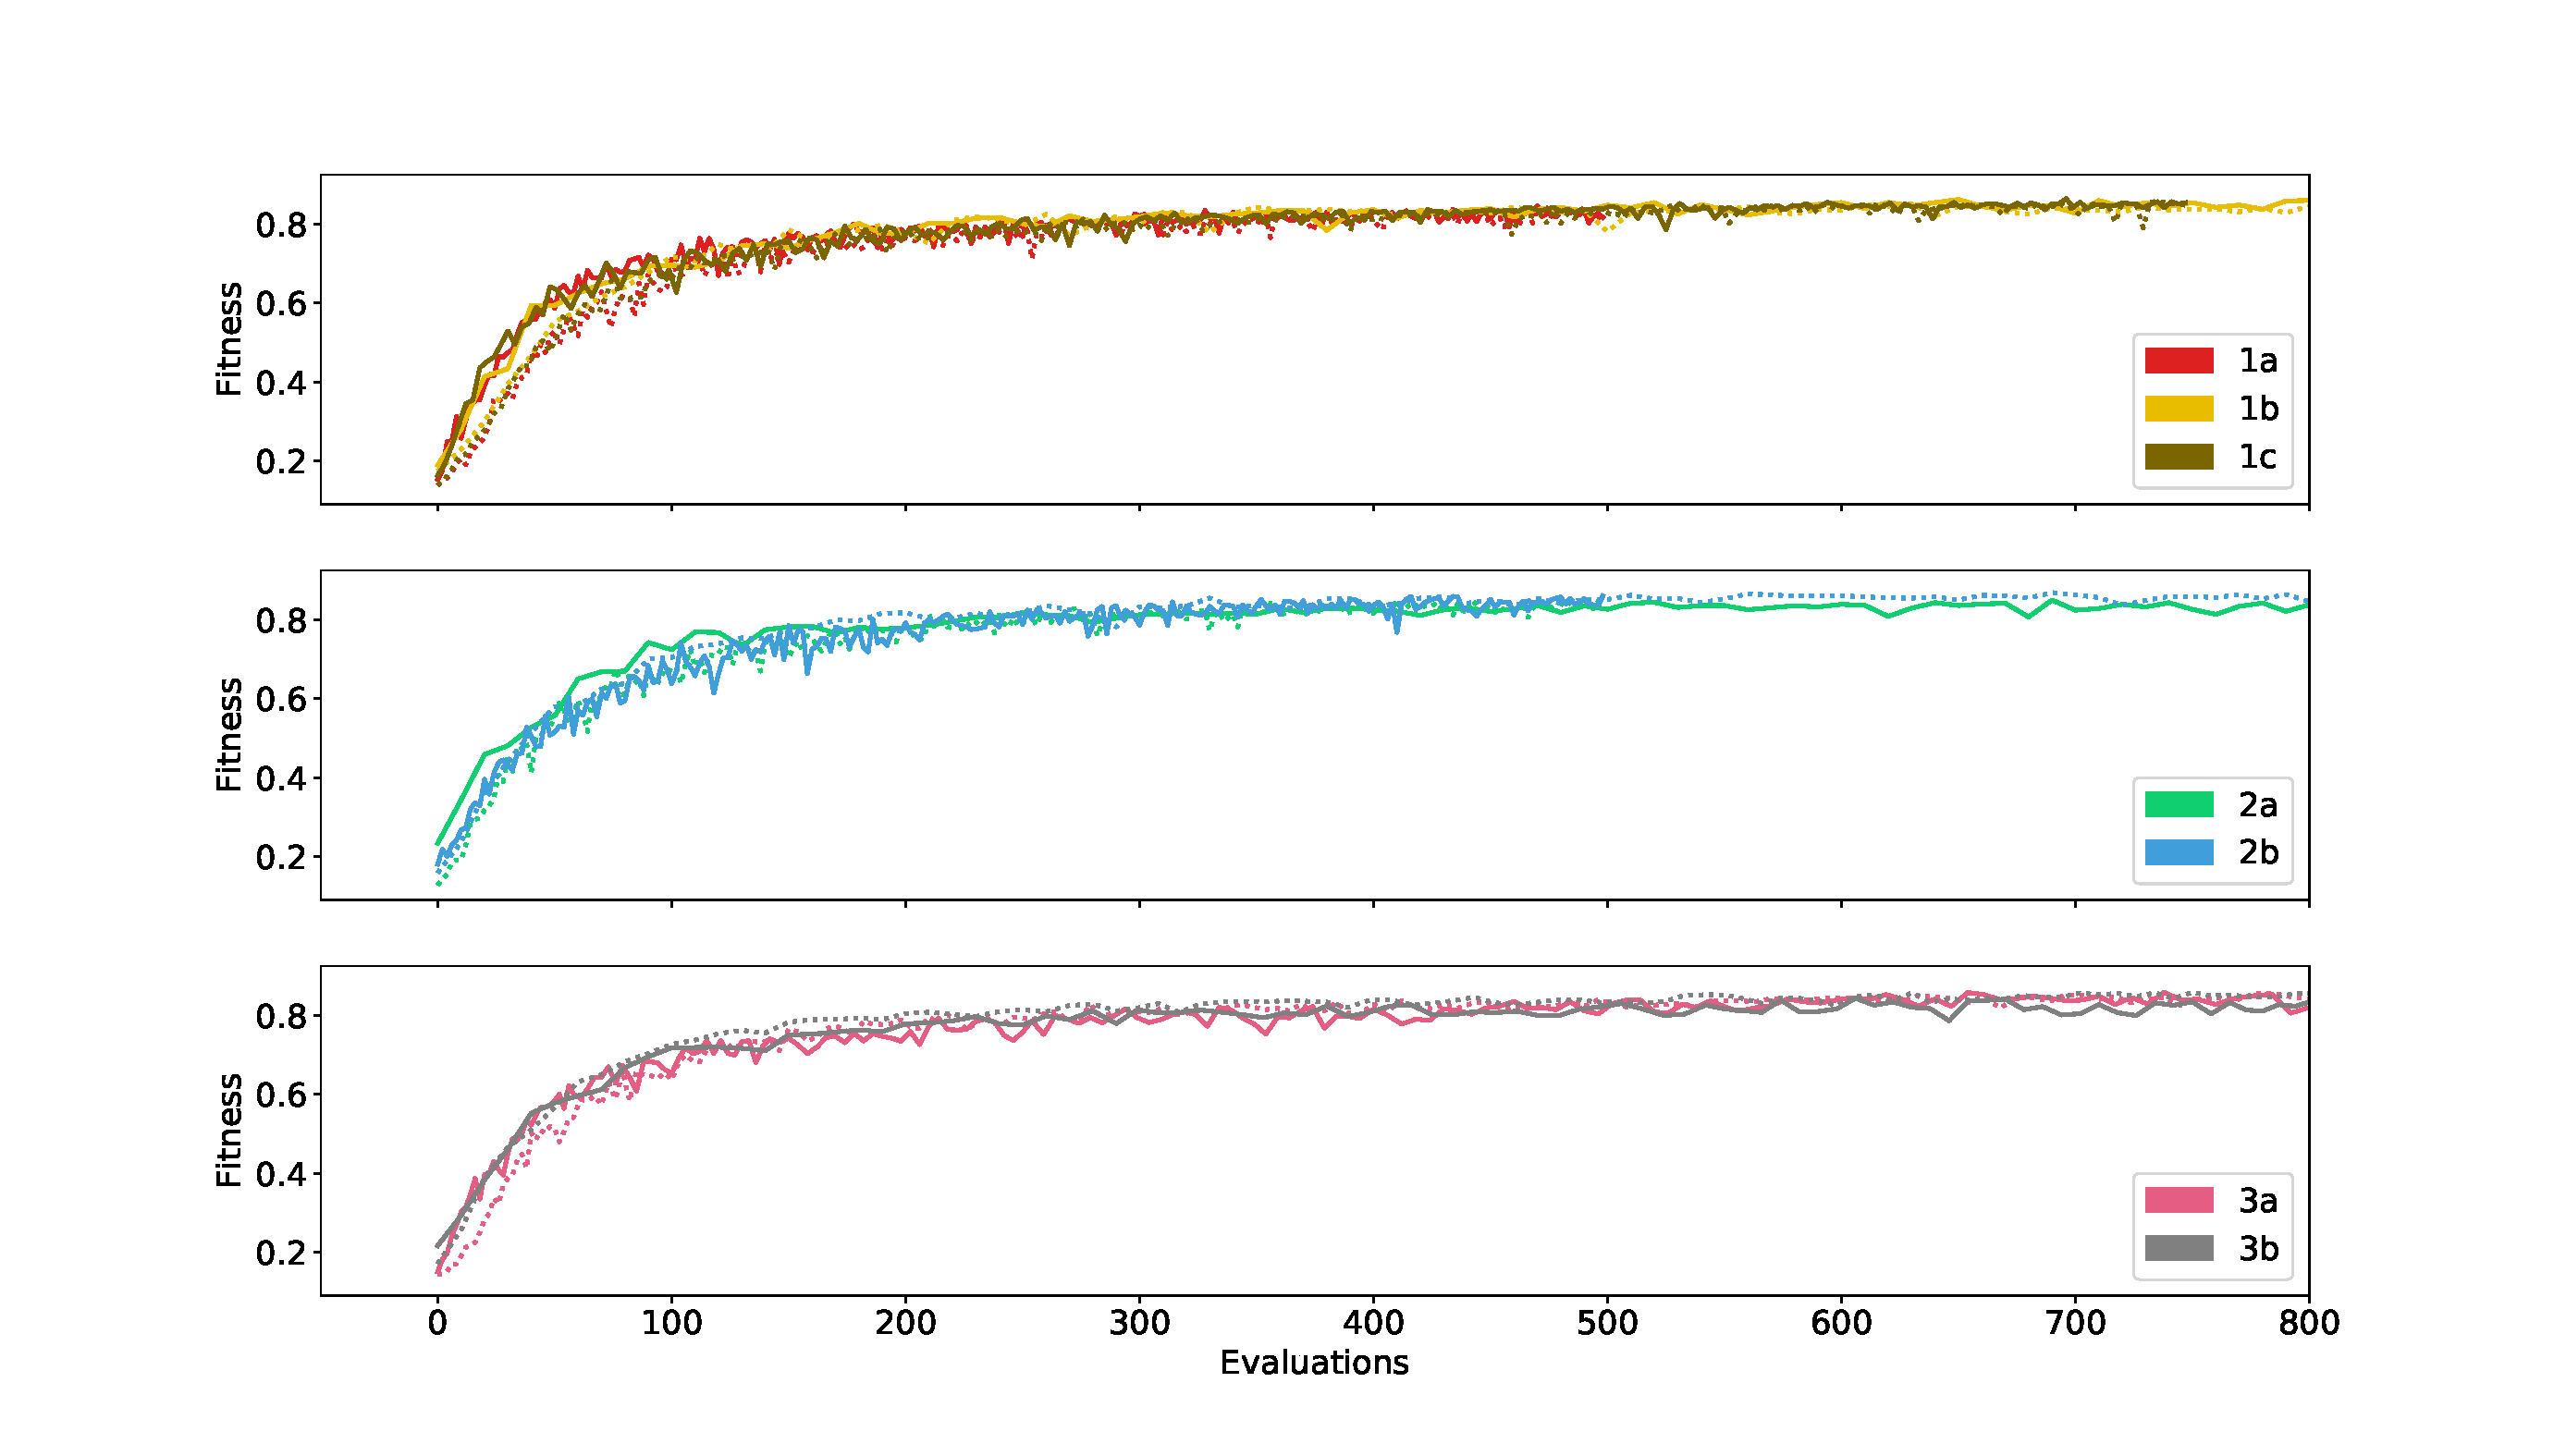
\includegraphics[width=1.25\textwidth, center]{Chapters/4.Experiments/exp3/figures/fitness_by_evaluations.pdf}
    \caption[Average tournament fitness plotted by evaluation]{The average tournament fitness as it changes with respect to number of evaluations for the first 800 evaluations. The dotted lines are average fitness during search for task 1, while the whole lines are for task 2.}
    \label{fig:exp3.fitness_by_evaluations}
\end{sidewaysfigure}

Figure \ref{fig:exp3.fitness} shows the average tournament fitness for each generation. As with results in chapter \ref{exp2}, the algorithms with high tournament size plateau in fitness quicker than algorithms with a low tournament size.

Noteworthy features of this plot are the increase in average fitness for algorithms with low tournament size in the start of each search from task 1 to task 2, suggesting the learning for these algorithms are easier the second time around. 

The plot in figure \ref{fig:exp3.fitness_by_evaluations} show the same progress in average tournament fitness, but here plotted by evaluation number and not generation. This figure shows us the increase in average fitness from task 1 to task 2 is not only for the low tournament size algorithms, but also that of algorithm 1b with a high tournament size for both tasks. This means the only algorithms with a similar fitness progression for both tasks is algorithms 2b and 3b. 

\section{Discussion}
As the searches themselves are the same as in chapter \ref{exp2}, the convergence rate of the different algorithms was not expected to be different from in chapter \ref{exp2}. However, the searches were run longer, and the figures \ref{fig:exp3.hamming} and \ref{fig:exp3.frequency} show a lengthened progression of the diversity than seen previously. Again the algorithms with large tournament size converge before 100 generations have passed, but the increase in generation limit gives algorithm 3a the time to reach a stable diversity level. We also noted that the recombination algorithm 1c converge significantly more for task 2 than task 1, implying that the convergence rate could be influenced by the reuse of modules. 

As expected from the experiments in this chapter, the level of modular reuse between tasks was higher than in chapter \ref{exp2}. This is clear from the comparison to the estimated module reuse when randomly selecting modules. In chapter \ref{exp2} we saw the reuse for all algorithms being significantly less than of random module selection, while this experiment shows reuse more than random module selection. Due to the smaller PathNet structure, and therefore smaller permutation space than in chapter \ref{exp2}, reusing modules is simpler. However, the reduction in permutation-space also increases the likelihood of randomly selecting a trained module during the Monte-Carlo estimation. The comparison to the random module selection ties the two experiments together, making us able to compare them. 

The only difference between task 1 and task 2 is that task 2 searches among modules where some contain trained parameters. The figures \ref{fig:exp3.fitness} and \ref{fig:exp3.fitness_by_evaluations} confirm then that reusing locked modules improves training as the average fitness of a tournament grows quicker for task 2. One can only assume this effect would get more prominent for a more complex task-domain where generalization is difficult and reusing knowledge becomes more valuable. 

\section{Conclusion}
These experiments do not provide any evidence for the different algorithms having any effect on the reuse of modules between tasks. As hypothesized, they did reach a higher module reuse than that of a random module selection, but as the conditions in this experiment were ideal for module reuse, this is not a huge feat.

The results do provide evidence for the reuse of modules influencing the search. As seen in figure \ref{fig:exp3.fitness} the fitness improve quicker when reusing trained modules. This is not surprising, however, as this was one of the motivations behind PathNet in the first place. What is surprising is the increased convergence rate for algorithm 1c during task 2. There is no conclusive proof of this being caused by reusing modules, but the only difference between the two searches are the presence of trained modules. This result calls for more testing to both confirm this result is replicable and the determine the cause. 